\documentclass[tikz,border=10pt]{standalone}
\usepackage{tkz-euclide} % 用于方便地处理几何图形

\begin{document}
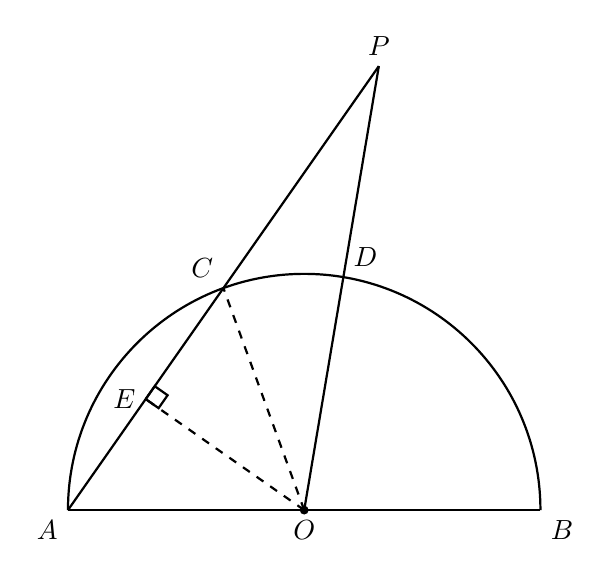
\begin{tikzpicture}[scale=2, thick, >=stealth]
    % 1. 定义基本参数和坐标点
    \coordinate (O) at (0,0);           % 圆心 O
    \coordinate (A) at (-1.5,0);        % 点 A
    \coordinate (B) at (1.5,0);         % 点 B
    
    % 定义点 C 在圆弧上 (大约 110 度位置)
    \coordinate (C) at ({1.5*cos(110)}, {1.5*sin(110)});
    
    % 2. 计算点 P 和 D 的位置
    % 延长 AC 到 P，这里设定 P 的位置
    \coordinate (P) at ($(A)!2!(C)$); 
    
    % 连接 OP 穿过圆弧交点为 D
    \path [name path=lineOP] (O) -- (P);
    \path [name path=arc] (1.5,0) arc (0:180:1.5);
    \path [name intersections={of=lineOP and arc, by=D}];

    % 3. 绘制图形边界
    % 绘制半圆直径 AB
    \draw (A) -- (B);
    % 绘制半圆弧
    \draw (1.5,0) arc (0:180:1.5);
    
    % 4. 绘制实线段
    \draw (A) -- (P); % 线段 AP
    \draw (O) -- (P); % 线段 OP
    
    % 5. 绘制辅助虚线
    \draw [dashed] (O) -- (C); % 辅助线 OC
    
    % 计算点 E: O 到 AC 的垂足
    \coordinate (E) at ($(A)!(O)!(C)$);
    \draw [dashed] (O) -- (E); % 辅助线 OE
    
    % 6. 标注直角符号
    \tkzMarkRightAngle[size=0.1](C,E,O)
    
    % 7. 标注顶点标签
    \node [below left] at (A) {$A$};
    \node [below right] at (B) {$B$};
    \node [below] at (O) {$O$};
    \node [above] at (P) {$P$};
    \node [above left] at (C) {$C$};
    \node [above right] at (D) {$D$};
    \node [left] at (E) {$E$};

    % 绘制圆心处的黑点
    \fill (O) circle (0.8pt);
\end{tikzpicture}
\end{document}